%% Ankur Sinha

%% packages %%
% support for coloured text
\usepackage{color}
% IPA
\usepackage{tipa}
\usepackage[scale=2]{ccicons}
\usepackage{amssymb}
\usepackage{tikz}
\usetikzlibrary{mindmap, arrows.meta, positioning, arrows}
\usepackage{pgfplots}
% Define the colours we use for E and I in all graphs
\definecolor{SinhaBlueE}{HTML}{3b4cc0}
\definecolor{SinhaRedI}{HTML}{f7a789}
\pgfmathdeclarefunction{gaussnew}{4}{%nu, eta, eps, omega
  \pgfmathparse{(#1*((2*exp(-(((x-((#2+#3)/2))/((#2-#3)/(2*sqrt(-ln(#4/2)))))^2))) -#4))}%chktex 36
}
\usepackage{jneurosci}
\usepackage{subfig}
\usepackage[T1]{fontenc}
\usepackage[utf8]{inputenc}
\usepackage[style=nature,backend=biber,autocite=footnote]{biblatex}
\addbibresource{/home/asinha/Documents/01_Readables/00_research_papers/masterbib.bib}
% Use opensans
% \usepackage[default,scale=0.95]{opensans}
\usepackage[sfdefault]{roboto}
% for strike through
\usepackage[normalem]{ulem}
% links, urls, refs
\definecolor{links}{HTML}{2A1B81}
% Fedora blue for the theme
\definecolor{FedoraBlue}{HTML}{2A1B81}
\usepackage{hyperref}
\hypersetup{colorlinks,linkcolor=Green,urlcolor=links}
% graphics
\usepackage{graphicx}
% algorithm
\usepackage{algorithmic}
\usepackage{textcomp}
\usepackage{wrapfig}
\usepackage{textgreek}
\usepackage{euler}
\usepackage{csquotes}

% beamer theme
% use defaults for theme
\usetheme[numbering=fraction]{metropolis}
\usefonttheme[onlymath]{serif}
\setbeamerfont{footnote}{size=\tiny}
\setbeamerfont{caption}{size=\tiny}
\setbeamercolor{alerted text}{fg=Green}
\setbeamerfont{note page}{size=\small}

% Not needed in metropolis, but in general footnote citation fixes: https://tex.stackexchange.com/questions/44217/how-can-i-stop-footcite-from-hijacking-my-beamer-columns
% how to use multiple references to the same footnote: https://tex.stackexchange.com/questions/27763/beamer-multiple-references-to-the-same-footnote

% Disable footnoterule
\renewcommand{\footnoterule}{}

%% title %%
\title{Investigating structural plasticity in brain networks using computational modelling}
\author[Ankur Sinha]{Ankur Sinha\\PhD candidate\\Biocomputation Research Group\\University of Hertfordshire.}
\date{17/01/2020}

%% document begins %%
\begin{document}


% title frame %%
\begin{frame}
  \titlepage{}
\end{frame}

%% Three slides for 5 minutes seems good
%% So, 30 slides at most for 50 minutes
\section{Context: what and why?}
\begin{frame}[c]{The plastic---but stable---brain: Hebbian/Homeostatic plasticity}
  \pause{}
  \begin{itemize}
    \item \enquote{Neurons that fire together, wire together.}\footnotemark[1]{}
      \pause{}
    \item \enquote{The more things change, the more they stay the same.}\footnotemark[2]{}
  \end{itemize}
  \footnotetext[1]<2->{\fullcite{Hebb1949}}
  \footnotetext[2]<3->{\fullcite{Turrigiano1999}}
\end{frame}
\begin{frame}[c]{Synaptic plasticity: the popular plasticity}
  \begin{itemize}
    \item changes in efficacy of \alert{existing} synapses,
      \pause{}
    \item changes in structure are ignored\footnote[1]{Even though structural changes in spines and boutons underlie modulation of synaptic efficacy.}.
  \end{itemize}
\end{frame}
\begin{frame}[c]{What underlies large scale reorganisation?}
  \begin{itemize}
    \item \fullcite{Rasmusson1982}
  \pause{}
  \scriptsize{
      \item \fullcite{Wall1984}
      \item \fullcite{Merzenich1984}
      \item \fullcite{Calford1988}
      \item \fullcite{Heinen1991}
      \item \fullcite{Rajan1993}
      }
  \end{itemize}
\end{frame}
\begin{frame}[c]{Two possible theories}
  \begin{itemize}
    \item \enquote{unmasking} of pre-existing synaptic connections,
      \pause{}
    \item formation of new synapses (\alert{structural plasticity}).
  \end{itemize}
  \footnotetext[1]{\fullcite{Rasmusson1982}}
\end{frame}
\begin{frame}[c]{Imaging confirms structural plasticity in lesion studies}
    \begin{itemize}
      \item \fullcite{Darian-Smith1994}
        \pause{}
        \footnotesize{
      \item \fullcite{Florence1998}
      \item \fullcite{Keck2008}
      \item \fullcite{Keck2011}
      \item \fullcite{Marik2014}
      }
    \end{itemize}
\end{frame}
\begin{frame}[c]{Also confirms structural plasticity in the unlesioned adult brain}
    \begin{itemize}
      \item \fullcite{Holtmaat2005}
        \pause{}
        \footnotesize{
      \item \fullcite{Stettler2006}
      \item \fullcite{Marik2010}
      \item \fullcite{Chen2012}
      \item \fullcite{Villa2016}
      }
    \end{itemize}
\end{frame}
\begin{frame}[c]{So:}
  \begin{itemize}
    \item not only do the strengths of existing synapses change,
    \item \alert{whole synapses are formed and removed.}
      \pause{}
    \item How? Why?
  \end{itemize}
\end{frame}
\begin{frame}[c]{Aim}
  \begin{center}
    \textbf{Simulate a computational model of peripheral lesioning to study the reorganisation process.}
  \end{center}
  \pause{}
  \begin{itemize}
    \item A computational model allows us to:
      \begin{itemize}
        \item investigate every entity in the network: variables from neurons, their neurites, and all synapses,
        \item modify any parameters to analyse changes in network behaviour: neuronal parameters, synaptic parameters,
        \item run multiple analyses in parallel,
        \item do it in less time than biological experiments\footnote[1]<2->{Simulations still take a week each, but that's still faster than a multi-month laboratory experiment.}.
      \end{itemize}
  \end{itemize}
\end{frame}
\section{Methods: How?}
\begin{frame}[c]{Peripheral lesion protocol I:\ topographic mapping}
  \note[item]{The protocol is pretty standard. Here, for a study in the visual cortex, the retinal field of a rat or a mouse is mapped.}
  \begin{columns}
    \begin{column}{0.5\textwidth}
      \centering
      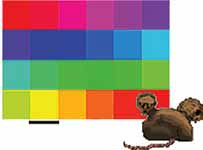
\includegraphics[width=0.8\textwidth]{99_images/keck-1-1a}%chktex 8
    \end{column}
    \begin{column}{0.5\textwidth}
      \centering
      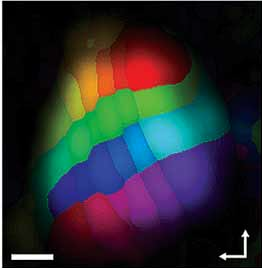
\includegraphics[width=0.8\textwidth]{99_images/keck-1-1c}%chktex 8
    \end{column}
  \end{columns}
  \footnotetext[1]{\fullcite{Keck2008}}
\end{frame}
\begin{frame}[c]{Peripheral lesion protocol II:\ after peripheral lesion}
  \note[item]{Then, a part of the retina is lesioned. This cuts off inputs to a part of the visual cortex, as shown in the first figure. This forms the Lesion Projection Zone (LPZ). By repeated imaging of the region over months, the reorganisation of the network is tracked.}
  \note[item]{Other lesion studies use similar methods: digit removal, whisker trimming, and so on---anything that cuts off projecting activity on to a set of neurons.}
  \begin{figure}[h]
    \centering
    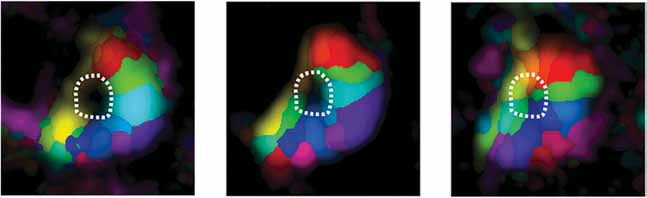
\includegraphics[width=\textwidth]{99_images/keck-1-2c}%chktex 8
  \end{figure}
  \begin{itemize}
    \item Dotted region encloses the Lesion Projection Zone (LPZ)
    \item Inward \enquote{repair}.
  \end{itemize}
    \footnotetext[1]{\fullcite{Keck2008}}
\end{frame}
\begin{frame}[c]{Data gathered from these experiments: summary}
  \note[item]{So, if this a simple schematic, of the regions around the LPZ, this is what we know from these studies.}
  \begin{columns}
    \begin{column}{0.3\textwidth}
      \centering
      \def\radiuscircle{0.6cm}
\begin{tikzpicture}[scale=0.8, transform shape]
  \fill [fill=black, thick, opacity=0.10] (0,0) rectangle ++(5,7.5);
  \node [below, black] at (3.5, 1.0){Other};

  \fill [cyan, opacity=1.0] (2.5, 3.5) circle (3.0*\radiuscircle);
  \draw [cyan, very thick] (1.5, 1.0)--(2.5, 3.5);
  \node [below, cyan] at (1.5, 1.0){Peri LPZ};

  \fill [black, opacity=1.0] (2.5, 3.5) circle (2.0*\radiuscircle);
  \draw [black, very thick] (1.5, 6.0)--(2.5, 3.5);
  \node [above, black] at (1.5, 6.0){LPZ B};

  \fill [green, opacity=1.0] (2.5, 3.5) circle (\radiuscircle);
  \draw [green, very thick] (3.5, 6.0)--(2.5, 3.5);
  \node [above, green] at (3.5, 6.0){LPZ C};

\end{tikzpicture}

    \end{column}
    \pause{}
    \begin{column}{0.6\textwidth}
      \begin{itemize}
        \item Inward repair of network.
        \item Massive disinhibition in the LPZ\@.
        \item Gradual \alert{ingrowth of excitatory synapses} from the peri-LPZ to the LPZ\@.
        \item Gradual \alert{outgrowth of inhibitory synapses} from the LPZ to the peri-LPZ\@.
      \end{itemize}
    \end{column}
  \end{columns}
\end{frame}
\begin{frame}[c]{Physiological cortical spiking network model}
  \begin{figure}[h]
    \def\svgwidth{0.7\textwidth}
    %% Creator: Inkscape inkscape 0.92+devel, www.inkscape.org
%% PDF/EPS/PS + LaTeX output extension by Johan Engelen, 2010
%% Accompanies image file 'schematic.eps' (pdf, eps, ps)
%%
%% To include the image in your LaTeX document, write
%%   \input{<filename>.pdf_tex}
%%  instead of
%%   \includegraphics{<filename>.pdf}
%% To scale the image, write
%%   \def\svgwidth{<desired width>}
%%   \input{<filename>.pdf_tex}
%%  instead of
%%   \includegraphics[width=<desired width>]{<filename>.pdf}
%%
%% Images with a different path to the parent latex file can
%% be accessed with the `import' package (which may need to be
%% installed) using
%%   \usepackage{import}
%% in the preamble, and then including the image with
%%   \import{<path to file>}{<filename>.pdf_tex}
%% Alternatively, one can specify
%%   \graphicspath{{<path to file>/}}
%% 
%% For more information, please see info/svg-inkscape on CTAN:
%%   http://tug.ctan.org/tex-archive/info/svg-inkscape
%%
\begingroup%
  \makeatletter%
  \providecommand\color[2][]{%
    \errmessage{(Inkscape) Color is used for the text in Inkscape, but the package `color.sty' is not loaded}%
    \renewcommand\color[2][]{}%
  }%
  \providecommand\transparent[1]{%
    \errmessage{(Inkscape) Transparency is used (non-zero) for the text in Inkscape, but the package `transparent.sty' is not loaded}%
    \renewcommand\transparent[1]{}%
  }%
  \providecommand\rotatebox[2]{#2}%
  \ifx\svgwidth\undefined%
    \setlength{\unitlength}{841.88976378bp}%
    \ifx\svgscale\undefined%
      \relax%
    \else%
      \setlength{\unitlength}{\unitlength{} * \real{\svgscale}}%
    \fi%
  \else%
    \setlength{\unitlength}{\svgwidth}%
  \fi%
  \global\let\svgwidth\undefined%
  \global\let\svgscale\undefined%
  \makeatother%
  \begin{picture}(1,0.8)(0,-0.1)%
    \put(0,0.05){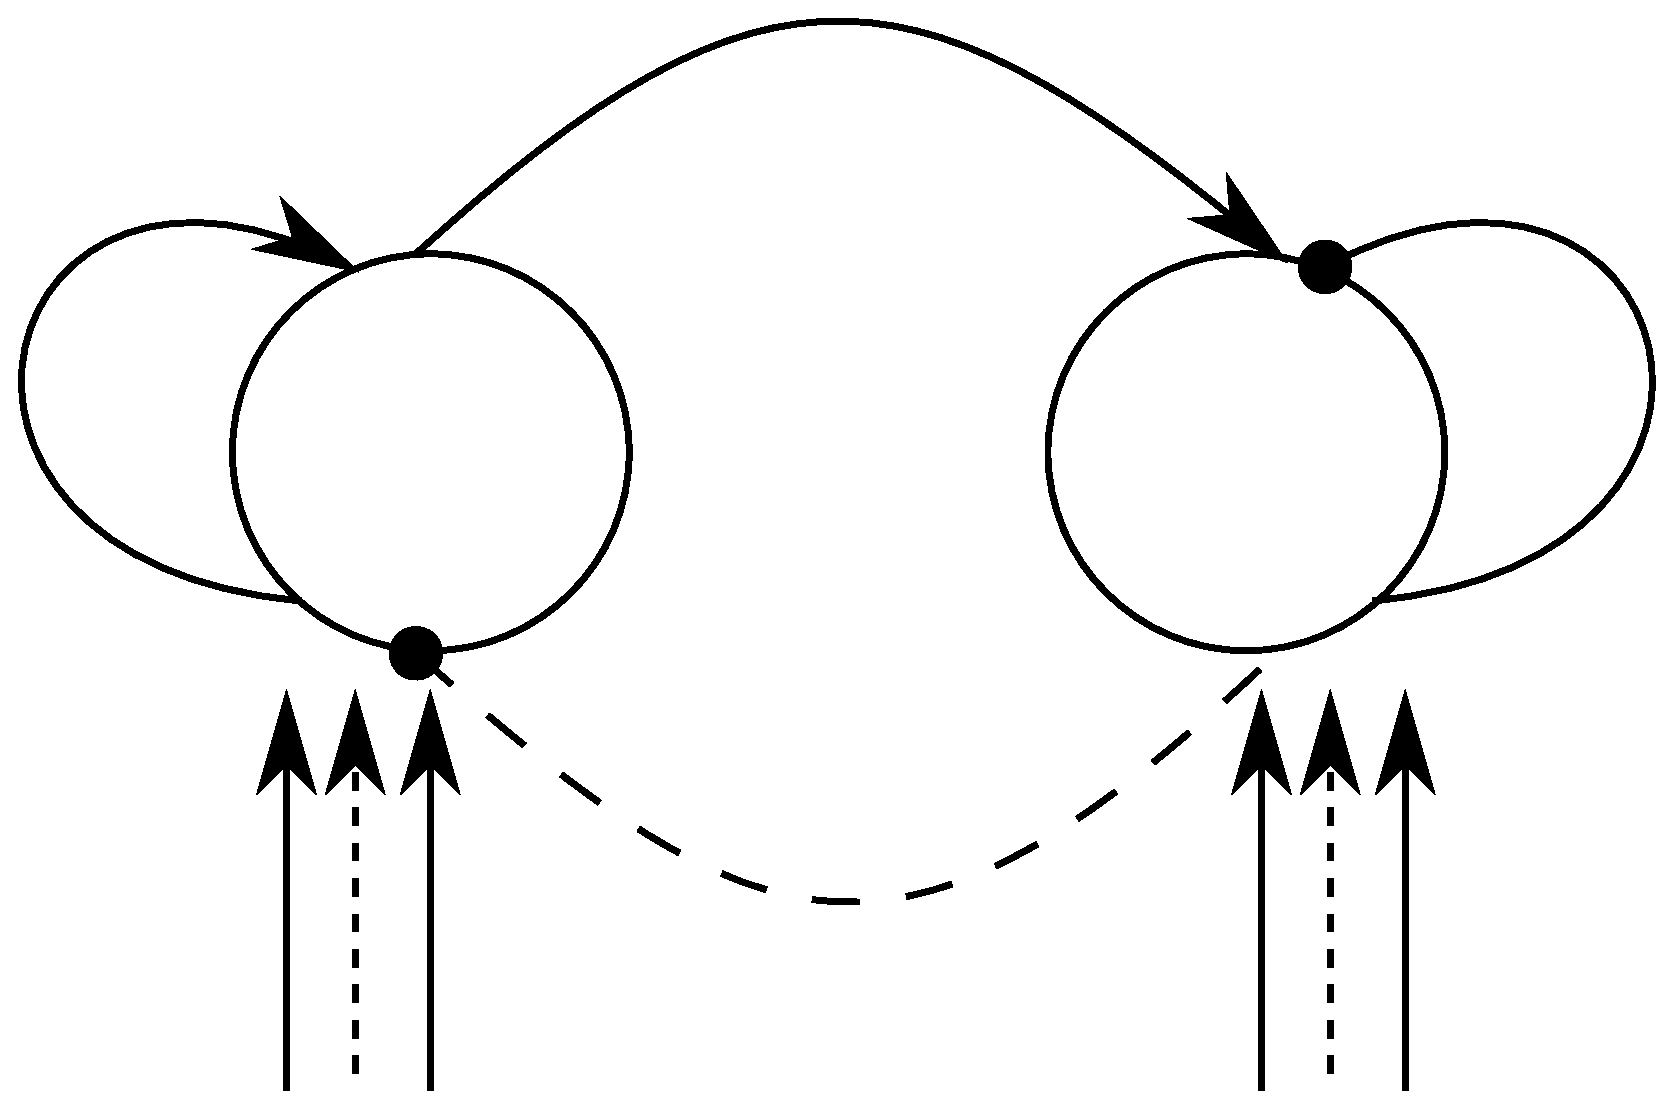
\includegraphics[width=\unitlength]{99_images/schematic.eps}}%
    \put(0.2347176,0.44870591){\color[rgb]{0,0,0}\makebox(0,0)[lb]{\smash{E}}}%
    \put(0.1747176,0.40870591){\color[rgb]{0,0,0}\makebox(0,0)[lb]{\smash{neurons}}}%
    \put(0.73973984,0.44870591){\color[rgb]{0,0,0}\makebox(0,0)[lb]{\smash{I}}}%
    \put(0.66973984,0.40870591){\color[rgb]{0,0,0}\makebox(0,0)[lb]{\smash{neurons}}}%
    \put(0.00355224,0.58941411){\color[rgb]{0,0,0}\makebox(0,0)[lb]{\smash{\(g_{EE}\)}}}%
    \put(0.46685226,0.65011583){\color[rgb]{0,0,0}\makebox(0,0)[lb]{\smash{\(g_{EI}\)}}}%
    \put(0.94063961,0.58941411){\color[rgb]{0,0,0}\makebox(0,0)[lb]{\smash{\(g_{II}\)}}}%
    \put(0.45717629,0.09520415){\color[rgb]{0,0,0}\makebox(0,0)[lb]{\smash{\(\textcolor{Red}{g_{IE}}\)}}}%
    \put(0.05,0.09520415){\color[rgb]{0,0,0}\makebox(0,0)[lb]{\smash{\(g_{ext}^E\)}}}%
    \put(0.86,0.09520415){\color[rgb]{0,0,0}\makebox(0,0)[lb]{\smash{\(g_{ext}^I\)}}}%
    \put(0.08028497,0.00){\color[rgb]{0,0,0}\makebox(0,0)[lb]{\smash{Ext stimulus}}}%
    \put(0.68617882,0.00){\color[rgb]{0,0,0}\makebox(0,0)[lb]{\smash{Ext stimulus}}}%
  \end{picture}%
\endgroup%


  \end{figure}
  \footnotetext[1]{\fullcite{Vogels2011}}
\end{frame}
\begin{frame}[t]{Neuron model: 8000 E, 2000 I neurons}
  \begin{columns}
    \begin{column}{0.6\textwidth}
      \begin{itemize}
        \item Point \enquote{leaky integrate and fire neurons}\footnotemark[1]{}, 
        \item Bear neurites (\(z\)).
      \end{itemize}
    \end{column}
    \begin{column}{0.4\textwidth}
      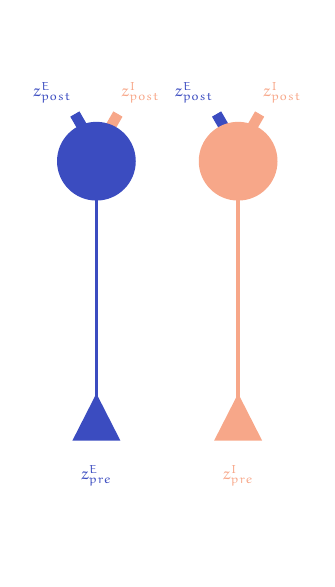
\begin{tikzpicture}[scale=0.6, transform shape]
  % Make it 12 cm long
  \node (O) at (0cm, 0cm) {};
  \node (L) at (0cm, -11cm) {};


  \node (E) at (0, -2cm) {};
  \node (I) at (3cm, -2cm) {};
  %end point of axons
  \node (axE) at (0, -8.5cm) {};
  \node (axI) at (3cm, -8.5cm) {};

  % post-elements E
  \draw [draw=SinhaBlueE, fill=SinhaBlueE, rotate around={30:(0cm,-2.5cm)}] (-0.1cm, -2.5cm) rectangle (0.1cm, -1.6cm);
  \draw [draw=SinhaRedI, fill=SinhaRedI, rotate around={-30:(0cm,-2.5cm)}] (-0.1cm, -2.5cm) rectangle (0.1cm, -1.6cm);
  \node [above left=0.4cm of E, text=SinhaBlueE] {\(z^E_{post}\)};
  \node [above right=0.4cm of E, text=SinhaRedI] {\(z^I_{post}\)};
  \node [below =0.4cm of axE, text=SinhaBlueE] {\(z^E_{pre}\)};

  % post-elements I
  \draw [draw=SinhaBlueE, fill=SinhaBlueE, rotate around={30:(3cm,-2.5cm)}] (2.9cm, -2.5cm) rectangle (3.1cm, -1.6cm);
  \draw [draw=SinhaRedI, fill=SinhaRedI, rotate around={-30:(3cm,-2.5cm)}] (2.9cm, -2.5cm) rectangle (3.1cm, -1.6cm);
  \node [above left=0.4cm of I, text=SinhaBlueE] {\(z^E_{post}\)};
  \node [above right=0.4cm of I, text=SinhaRedI] {\(z^I_{post}\)};
  \node [below =0.4cm of axI, text=SinhaRedI] {\(z^I_{pre}\)};

  % axons later so they overlap the dendritic bits
  \draw[draw=SinhaBlueE, {Circle[width=1.0cm, length=1.0cm]}-{Triangle[reversed, length=6mm, width=6mm]}, very thick, fill=SinhaBlueE] (E.north) -- (axE.south);
  \draw[draw=SinhaRedI, {Circle[width=1.0cm, length=1.0cm]}-{Triangle[reversed, length=6mm, width=6mm]}, very thick, fill=SinhaRedI] (I.north) -- (axI.south);
\end{tikzpicture}

    \end{column}
  \end{columns}
  \footnotetext[1]{\fullcite{Meffin2004}}
\end{frame}
\begin{frame}[t]{Modelling synapse formation and removal}
  \begin{columns}
    \begin{column}{0.6\textwidth}
      \begin{itemize}
        \item \(z^E_{post} + z^E_{pre}\)
        \item \(z^I_{post} + z^I_{pre}\)
        \item New synapses form when \alert{free} partner neurites are available.
        \item Synapses are deleted if neurites are \alert{retracted} by the neuron.
      \end{itemize}
    \end{column}
    \begin{column}{0.4\textwidth}
      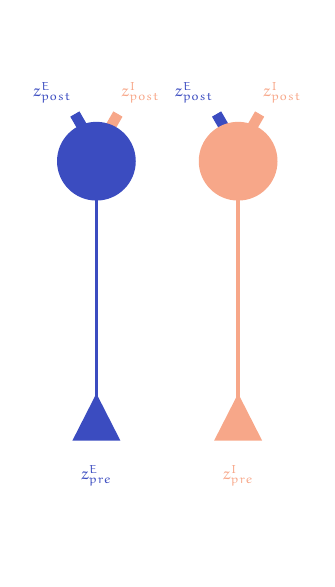
\begin{tikzpicture}[scale=0.6, transform shape]
  % Make it 12 cm long
  \node (O) at (0cm, 0cm) {};
  \node (L) at (0cm, -11cm) {};


  \node (E) at (0, -2cm) {};
  \node (I) at (3cm, -2cm) {};
  %end point of axons
  \node (axE) at (0, -8.5cm) {};
  \node (axI) at (3cm, -8.5cm) {};

  % post-elements E
  \draw [draw=SinhaBlueE, fill=SinhaBlueE, rotate around={30:(0cm,-2.5cm)}] (-0.1cm, -2.5cm) rectangle (0.1cm, -1.6cm);
  \draw [draw=SinhaRedI, fill=SinhaRedI, rotate around={-30:(0cm,-2.5cm)}] (-0.1cm, -2.5cm) rectangle (0.1cm, -1.6cm);
  \node [above left=0.4cm of E, text=SinhaBlueE] {\(z^E_{post}\)};
  \node [above right=0.4cm of E, text=SinhaRedI] {\(z^I_{post}\)};
  \node [below =0.4cm of axE, text=SinhaBlueE] {\(z^E_{pre}\)};

  % post-elements I
  \draw [draw=SinhaBlueE, fill=SinhaBlueE, rotate around={30:(3cm,-2.5cm)}] (2.9cm, -2.5cm) rectangle (3.1cm, -1.6cm);
  \draw [draw=SinhaRedI, fill=SinhaRedI, rotate around={-30:(3cm,-2.5cm)}] (2.9cm, -2.5cm) rectangle (3.1cm, -1.6cm);
  \node [above left=0.4cm of I, text=SinhaBlueE] {\(z^E_{post}\)};
  \node [above right=0.4cm of I, text=SinhaRedI] {\(z^I_{post}\)};
  \node [below =0.4cm of axI, text=SinhaRedI] {\(z^I_{pre}\)};

  % axons later so they overlap the dendritic bits
  \draw[draw=SinhaBlueE, {Circle[width=1.0cm, length=1.0cm]}-{Triangle[reversed, length=6mm, width=6mm]}, very thick, fill=SinhaBlueE] (E.north) -- (axE.south);
  \draw[draw=SinhaRedI, {Circle[width=1.0cm, length=1.0cm]}-{Triangle[reversed, length=6mm, width=6mm]}, very thick, fill=SinhaRedI] (I.north) -- (axI.south);
\end{tikzpicture}

    \end{column}
  \end{columns}
\end{frame}
\begin{frame}[t]{Model core: activity dependent neurite growth (\(z\))}
  \vspace{0.4cm}
  \begin{columns}
    \begin{column}{0.5\textwidth}
      \centering
      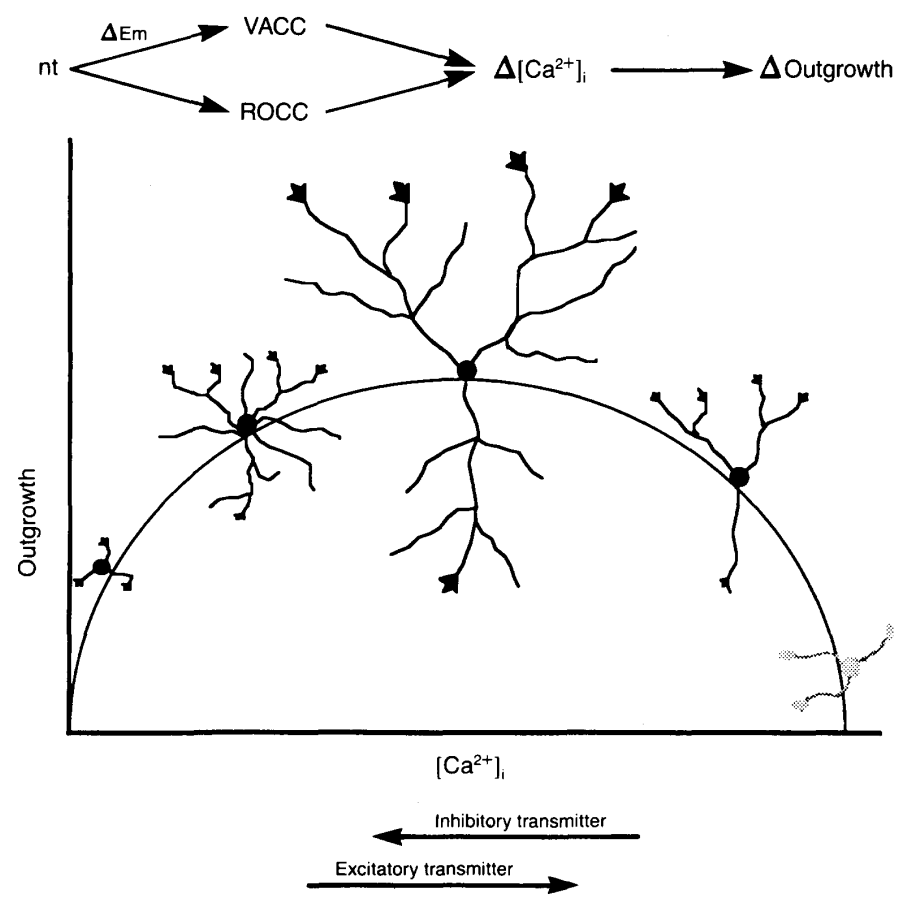
\includegraphics[width=0.9\textwidth]{99_images/lipton1989.png}%chktex 8
    \end{column}
    \pause{}
    \begin{column}{0.5\textwidth}
      \centering
      \begin{tikzpicture}[scale=1, transform shape]
    \begin{axis}[
      no markers, domain=-0:20, samples=100,
      x label style={at={(axis cs:10,-1.0)}},
      y label style={rotate=-90},
      x axis line style={->},
      y axis line style={<->},
      ymin=-1.5, ymax=2.0,
      axis x line*=center,
      axis y line*=left,
      xlabel={\([Ca^{2+}]\)}, ylabel={\(\frac{dz}{dt}\)},
      grid=major, ytick={-1,0,1}, xtick=\empty, clip=false,
      axis on top,
      height=6cm, width=\textwidth, enlargelimits=false
      ]
      % excitatory dendritic elements
      \addplot [very thick] {gaussnew(1,5.0, 15.0, 1.0)};

      \node[left ] (X) at (axis cs:0.0, 1.5) {}; % add to increase some space on top
      % \node[above left] (E) at (axis cs:5., 0.0000){\(\eta\)};
      % \node[above right] (F) at (axis cs:15., 0.0000){\(\epsilon\)};

      \draw [thick, dashed, -] (axis cs:5.0, -1.5)--(axis cs:5.0, 1.7);
      \node [above] at (axis cs:5.0, 1.7){\(\psi\)};

    \end{axis}
  \end{tikzpicture}


    \end{column}
  \end{columns}
  \footnotetext[1]{\fullcite{Lipton1989}}
  \footnotetext[2]<2->{\fullcite{Butz2013}}
\end{frame}
\begin{frame}[t]{Growth curves: possibilities}
  \vspace{0.4cm}
  \begin{columns}
    \begin{column}{0.5\textwidth}
      \centering
      \begin{tikzpicture}[scale=1, transform shape]
    \begin{axis}[
      no markers, domain=-0:20, samples=100,
      x label style={at={(axis cs:10,-1.0)}},
      y label style={rotate=-90},
      x axis line style={->},
      y axis line style={<->},
      ymin=-1.5, ymax=2.0,
      axis x line*=center,
      axis y line*=left,
      xlabel={\([Ca^{2+}]\)}, ylabel={\(\frac{dz}{dt}\)},
      grid=major, ytick={-1,0,1}, xtick=\empty, clip=false,
      axis on top,
      height=6cm, width=\textwidth, enlargelimits=false
      ]
      % excitatory dendritic elements
      \addplot [very thick] {gaussnew(1,5.0, 15.0, 1.0)};

      \node[left ] (X) at (axis cs:0.0, 1.5) {}; % add to increase some space on top
      % \node[above left] (E) at (axis cs:5., 0.0000){\(\eta\)};
      % \node[above right] (F) at (axis cs:15., 0.0000){\(\epsilon\)};

      \draw [thick, dashed, -] (axis cs:5.0, -1.5)--(axis cs:5.0, 1.7);
      \node [above] at (axis cs:5.0, 1.7){\(\psi\)};

    \end{axis}
  \end{tikzpicture}


    \end{column}
    \begin{column}{0.5\textwidth}
      \centering
      \begin{tikzpicture}[scale=1, transform shape]
    \begin{axis}[
      no markers, domain=-0:20, samples=100,
      x label style={at={(axis cs:10,-1.0)}},
      y label style={rotate=-90},
      x axis line style={->},
      y axis line style={<->},
      ymin=-1.5, ymax=2.5,
      axis x line*=center,
      axis y line*=left,
      xlabel={\([Ca^{2+}]\)},
      ylabel={\(\frac{dz}{dt}\)},
      grid=major, ytick={-1,0,1}, xtick=\empty, clip=false,
      axis on top,
      height=6cm, width=\textwidth, enlargelimits=false
      ]
      % excitatory dendritic elements
      \addplot [very thick] {gaussnew(1,5.0, 15.0, 0.001)};

      \node[left ] (X) at (axis cs:0.0, 1.5) {}; % add to increase some space on top
      % \node[above left] (E) at (axis cs:5., 0.0000){\(\eta\)};
      % \node[above right] (F) at (axis cs:15., 0.0000){\(\epsilon\)};

      \draw [thick, dashed, -] (axis cs:15.0, -1.5)--(axis cs:15.0, 2.1);
      \node [above] at (axis cs:15.0, 2.2){\(\psi\)};
    \end{axis}
  \end{tikzpicture}


    \end{column}
  \end{columns}
  \begin{center}
    We must determine 6 sets of growth curves: 3 for E, 3 for I neurons. Each growth curve has 4 free parameters.
  \end{center}
  \footnotetext[1]{\fullcite{Sinha2019a}}
\end{frame}
\begin{frame}[c]{Replicate peripheral lesion protocol}
  \begin{figure}[h]
    \centering
    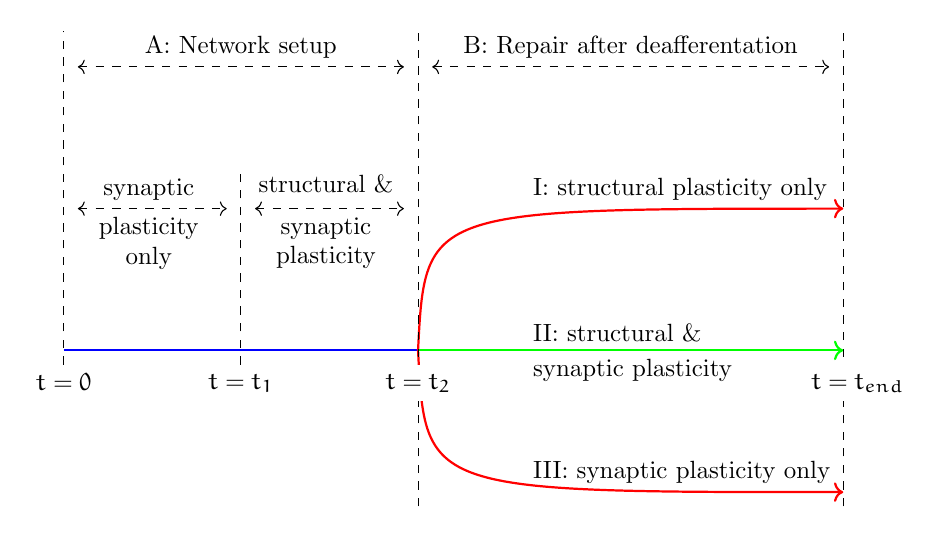
\begin{tikzpicture}[scale=0.9, transform shape]

  % horizontal lines
  \draw[blue, thick] (0,4) -- (5,4);
  \draw[green, thick, ->] (5,4) -- (11,4);
  \draw[red, thick, ->] (5,4) .. controls (5.1,6) .. (11,6);
  \draw[red, thick, ->] (5,4) .. controls (5.1,2) .. (11,2);


  \draw[dashed] (0,3.8) -- (0,8.5);
  \node[below] at (0, 3.8)  {\(t=0\)};

  \draw[dashed] (2.5,3.8) -- (2.5,6.5);
  \node[below] at (2.5, 3.8)  {\(t=t_1\)};

  \draw[dashed, -] (5,1.8) -- (5,8.5);
  \node[below, fill=white] at (5, 3.8)  {\(t=t_2\)};

  \draw[dashed] (11,1.8) -- (11,8.5);
  \node[below, fill=white] at (11.2, 3.8)  {\(t=t_{end}\)};

  \draw[dashed, <->] (0.2,8) -- (4.8,8);
  \node[above] at (2.5,8) {A: Network setup};

  \draw[dashed, <->] (0.2,6) -- (2.3,6);
  \node[above] at (1.2,6) {synaptic};
  \node[below, align=center] at (1.2,6) {plasticity\\only};
  \draw[dashed, <->] (2.7,6) -- (4.8,6);
  \node[above] at (3.7,6.1) {structural \&};
  \node[below, align=center] at (3.7,6) {synaptic\\plasticity};

  \draw[dashed, <->] (5.2,8) -- (10.8,8);
  \node[above] at (8,8) {B: Repair after deafferentation};


  \node[above right, align=left] at (6.5,6) {I: structural plasticity only};
  \node[above right, align=left] at (6.5,4) {II: structural \&};
  \node[below right, align=left] at (6.5,4) {synaptic plasticity};
  \node[above right, align=left] at (6.5,2) {III: synaptic plasticity only};

\end{tikzpicture}

  \end{figure}
\end{frame}
\section{Results and discussion}
\begin{frame}[c]{Deafferentation and successful repair}
  \begin{figure}
      \centering
      \resizebox{\textwidth}{!}{% GNUPLOT: LaTeX picture with Postscript
\begingroup
  \makeatletter
  \providecommand\color[2][]{%
    \GenericError{(gnuplot) \space\space\space\@spaces}{%
      Package color not loaded in conjunction with
      terminal option `colourtext'%
    }{See the gnuplot documentation for explanation.%
    }{Either use 'blacktext' in gnuplot or load the package
      color.sty in LaTeX.}%
    \renewcommand\color[2][]{}%
  }%
  \providecommand\includegraphics[2][]{%
    \GenericError{(gnuplot) \space\space\space\@spaces}{%
      Package graphicx or graphics not loaded%
    }{See the gnuplot documentation for explanation.%
    }{The gnuplot epslatex terminal needs graphicx.sty or graphics.sty.}%
    \renewcommand\includegraphics[2][]{}%
  }%
  \providecommand\rotatebox[2]{#2}%
  \@ifundefined{ifGPcolor}{%
    \newif\ifGPcolor
    \GPcolortrue
  }{}%
  \@ifundefined{ifGPblacktext}{%
    \newif\ifGPblacktext
    \GPblacktexttrue
  }{}%
  % define a \g@addto@macro without @ in the name:
  \let\gplgaddtomacro\g@addto@macro
  % define empty templates for all commands taking text:
  \gdef\gplbacktext{}%
  \gdef\gplfronttext{}%
  \makeatother
  \ifGPblacktext
    % no textcolor at all
    \def\colorrgb#1{}%
    \def\colorgray#1{}%
  \else
    % gray or color?
    \ifGPcolor
      \def\colorrgb#1{\color[rgb]{#1}}%
      \def\colorgray#1{\color[gray]{#1}}%
      \expandafter\def\csname LTw\endcsname{\color{white}}%
      \expandafter\def\csname LTb\endcsname{\color{black}}%
      \expandafter\def\csname LTa\endcsname{\color{black}}%
      \expandafter\def\csname LT0\endcsname{\color[rgb]{1,0,0}}%
      \expandafter\def\csname LT1\endcsname{\color[rgb]{0,1,0}}%
      \expandafter\def\csname LT2\endcsname{\color[rgb]{0,0,1}}%
      \expandafter\def\csname LT3\endcsname{\color[rgb]{1,0,1}}%
      \expandafter\def\csname LT4\endcsname{\color[rgb]{0,1,1}}%
      \expandafter\def\csname LT5\endcsname{\color[rgb]{1,1,0}}%
      \expandafter\def\csname LT6\endcsname{\color[rgb]{0,0,0}}%
      \expandafter\def\csname LT7\endcsname{\color[rgb]{1,0.3,0}}%
      \expandafter\def\csname LT8\endcsname{\color[rgb]{0.5,0.5,0.5}}%
    \else
      % gray
      \def\colorrgb#1{\color{black}}%
      \def\colorgray#1{\color[gray]{#1}}%
      \expandafter\def\csname LTw\endcsname{\color{white}}%
      \expandafter\def\csname LTb\endcsname{\color{black}}%
      \expandafter\def\csname LTa\endcsname{\color{black}}%
      \expandafter\def\csname LT0\endcsname{\color{black}}%
      \expandafter\def\csname LT1\endcsname{\color{black}}%
      \expandafter\def\csname LT2\endcsname{\color{black}}%
      \expandafter\def\csname LT3\endcsname{\color{black}}%
      \expandafter\def\csname LT4\endcsname{\color{black}}%
      \expandafter\def\csname LT5\endcsname{\color{black}}%
      \expandafter\def\csname LT6\endcsname{\color{black}}%
      \expandafter\def\csname LT7\endcsname{\color{black}}%
      \expandafter\def\csname LT8\endcsname{\color{black}}%
    \fi
  \fi
    \setlength{\unitlength}{0.0500bp}%
    \ifx\gptboxheight\undefined%
      \newlength{\gptboxheight}%
      \newlength{\gptboxwidth}%
      \newsavebox{\gptboxtext}%
    \fi%
    \setlength{\fboxrule}{0.5pt}%
    \setlength{\fboxsep}{1pt}%
\begin{picture}(22676.00,8502.00)%
    \gplgaddtomacro\gplbacktext{%
    }%
    \gplgaddtomacro\gplfronttext{%
      \csname LTb\endcsname%
      \put(359,170){\makebox(0,0)[l]{\strut{}$1$}}%
      \put(359,8458){\makebox(0,0)[l]{\strut{}$5$}}%
      \put(0,4314){\rotatebox{-270}{\makebox(0,0){\strut{}Firing rate (Hz)}}}%
    }%
    \gplgaddtomacro\gplbacktext{%
    }%
    \gplgaddtomacro\gplfronttext{%
    }%
    \gplgaddtomacro\gplbacktext{%
    }%
    \gplgaddtomacro\gplfronttext{%
    }%
    \gplbacktext
    \put(0,0){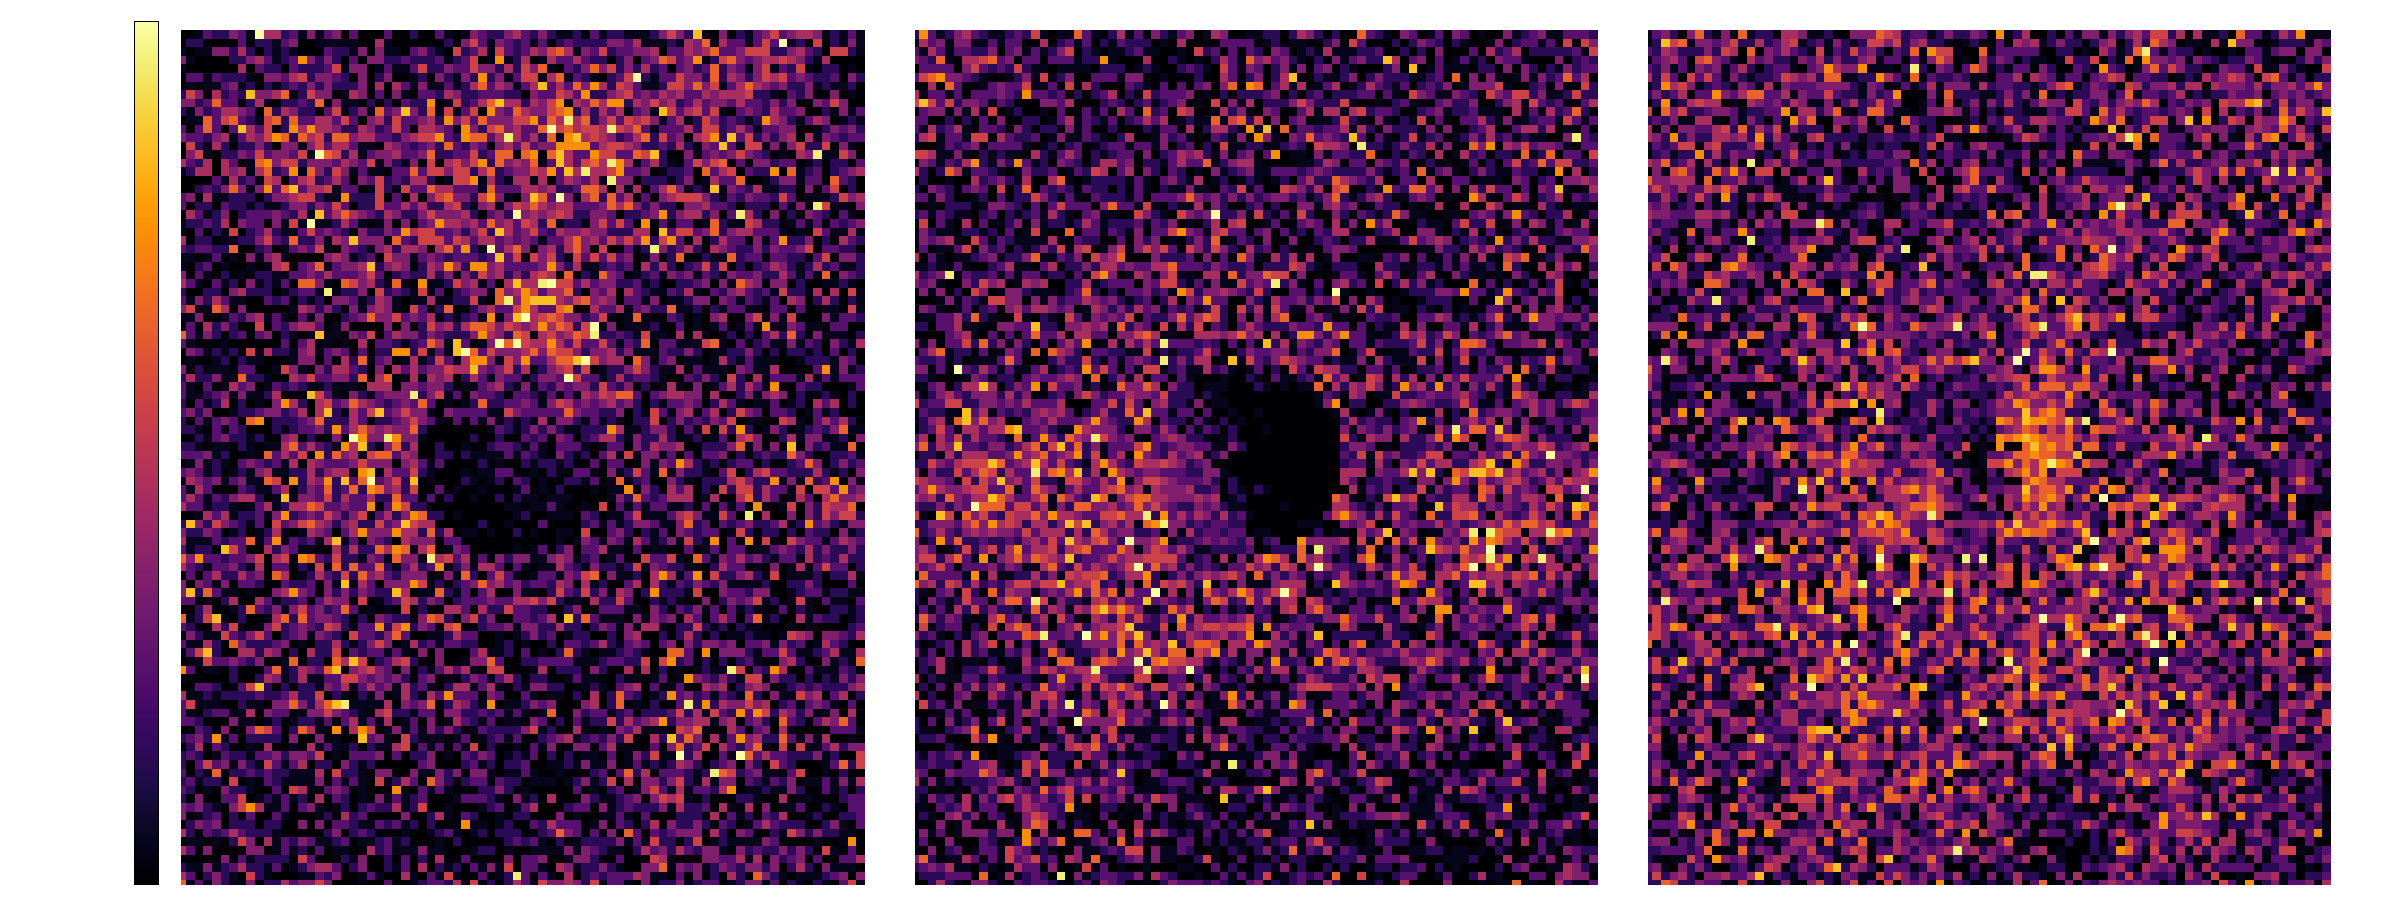
\includegraphics{99_images/201905131224-firing-rate-snapshots-E.eps}}%
    \gplfronttext
  \end{picture}%
\endgroup
}%
  \end{figure}
\end{frame}
\section{NeuroFedora: Free Software for Free Neuroscience}
